\documentclass[11pt]{article}
\usepackage[margin=1in]{geometry}
\usepackage{amsmath,amssymb,graphicx,array}
\usepackage[hidelinks]{hyperref}
\setlength{\parindent}{0pt}
\setlength{\parskip}{6pt}
\begin{document}
\begin{center}\Large Pricing conditions and comparative statics\end{center}
\section*{Notation and definitions}
We study one product and suppress its fixed index $j$: $p_{jt}$ becomes $p_t$
and $s_{jt}$ becomes $s_t$. The outside-option share $s_{0t}$ is
written as $1-s_t$. $v_t$ is systematic component of utility.

\renewcommand{\arraystretch}{1.25}
\begin{tabular}{@{}p{0.19\linewidth}p{0.76\linewidth}@{}}
\hline
Symbol & Definition \\
\hline
$t\in\{1,2\}$ & Time period. \\
$j$ & Fixed product index, suppressed in displayed formulas. \\
$p_t$, $p_t^*$ & Price and optimal price in period $t$, respectively. \\
$c\geq0$ & Constant marginal cost, common to both periods. \\
$v_t$ & Systematic utility from purchasing in period $t$; outside utility is zero. \\
$s_t\in(0,1)$ & Logit purchase probability. In period 2 this is conditional on a period-1 purchase. \\
$1-s_t$ & Probability of choosing the outside option in period $t$. \\
$\alpha<0$ & Price coefficient in utility; $-\alpha>0$ is price sensitivity. \\
$\beta$ & Baseline utility or demand intercept. \\
$\gamma$ & Utility coefficient on the history indicator, called switching preference in the figures. \\
$z_t\in\{0,1\}$ & Fixed, observed history indicator that shifts period-$t$ utility by $\gamma z_t$. \\
$\delta\in(0,1)$ & Discount factor on period-2 profit. \\
$\Pi$, $\Pi^*$ & Expected discounted profit per initial customer, and its optimized value. \\
$F_1$, $F_2$ & Period-1 profit derivative and normalized period-2 profit derivative; their roots give the pricing FOCs. \\
$R^*$ & Optimal price ratio $p_1^*/p_2^*$. \\
$\partial$, $\mathrm d$ & Partial derivatives hold the other price fixed; total derivatives allow both optimal prices and shares to adjust. \\
\hline
\end{tabular}

An asterisk denotes evaluation at the optimum. In all derivative formulas,
unstarred prices and shares on the right-hand side are evaluated at that optimum.

\[
\alpha=-2,\quad \beta=-1,\quad \delta=0.7,\quad c=1,\quad
(z_1,z_2)\in\{(0,0),(1,0),(0,1)\},\quad \gamma\in[0,3].
\]
\clearpage
\section{Symbolically derived equations}
Here $q_2=q(x_1)$, $s_2=s_2(x_1)$ and $p_2=p_2(x_1)$ describe a fixed terminal history. Price equations and comparative-static right-hand sides use equilibrium shares; the profit and FOCs use shares at the candidate prices.
\[
v_1 = \alpha p_{1} + \beta + \gamma q
\]
\[
v_2 = \alpha p_{2} + \beta + \gamma q_{2}
\]
\[
\Pi = \delta \left(V_{20} \left(1 - s\right) + V_{2j} s\right) + s \left(- c + p_{1}\right)
\]
\[
F_1 = \alpha s \left(1 - s\right) \left(- c + \delta \left(- V_{20} + V_{2j}\right) + p_{1}\right) + s
\]
\[
F_2 = \alpha s_{2} \left(1 - s_{2}\right) \left(- c + p_{2}\right) + s_{2}
\]
\[
p_1^* = c - \delta \left(- V_{20} + V_{2j}\right) - \frac{1}{\alpha \left(1 - s\right)}
\]
\[
p_2^* = c - \frac{1}{\alpha \left(1 - s_{2}\right)}
\]
\[
\frac{dp_1^*}{d\gamma} = \frac{\delta \left(s - 1\right) \left(u + v\right) - q s}{\alpha}
\]
\[
\frac{dp_2^*}{d\gamma} = - \frac{q_{2} s_{2}}{\alpha}
\]
\[
\frac{d\Pi^*}{d\gamma} = \frac{\delta \left(s u + v \left(s - 1\right)\right) - q s}{\alpha}
\]

\clearpage
\section*{Optimized expected profit}
\[
\Pi^* = \delta s_{1} s_{2} \left(- c + p_{2}\right) + s_{1} \left(- c + p_{1}\right)
\]
\begin{figure}[htbp]
\centering
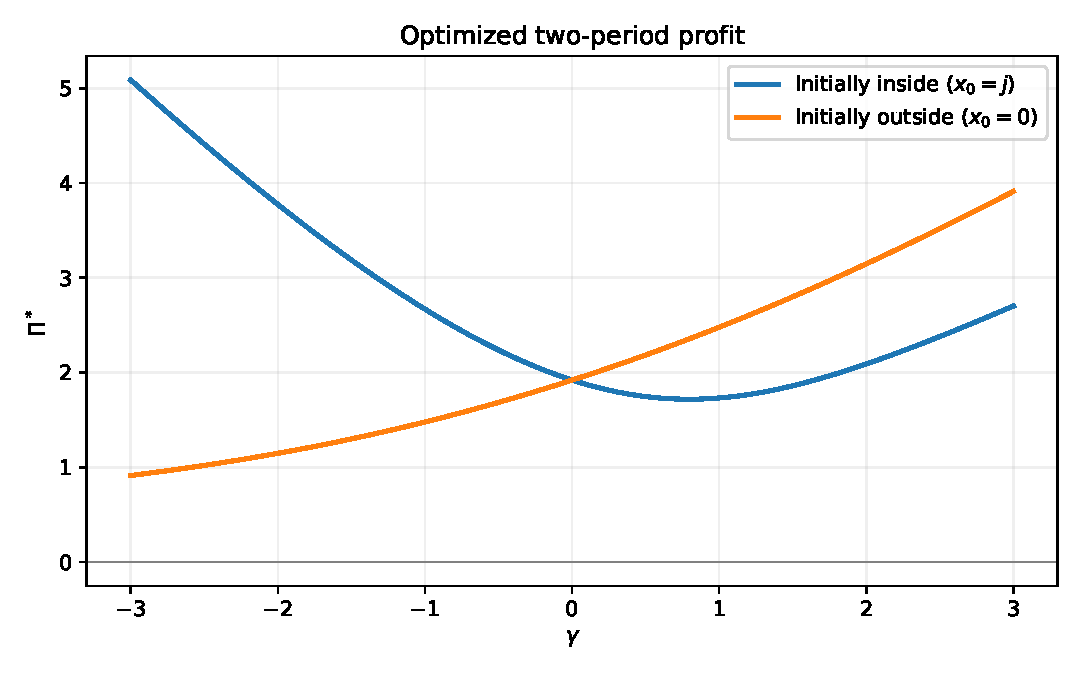
\includegraphics[width=\linewidth]{figures/profit_by_gamma.pdf}
\end{figure}
\clearpage
\section*{Optimal price ratio}
\[
R^* = \frac{p_{1}}{p_{2}}
\]
\begin{figure}[htbp]
\centering
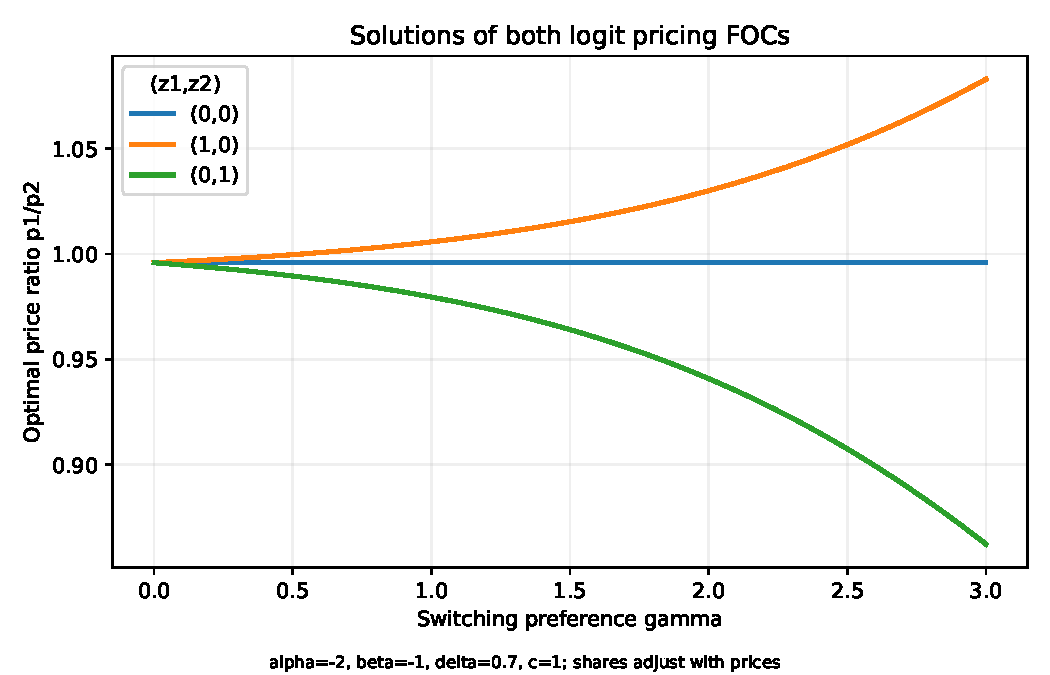
\includegraphics[width=\linewidth]{figures/price_ratio_by_gamma.pdf}
\end{figure}
\clearpage
\section*{Price-ratio derivative in gamma}
\[
\frac{\mathrm{d}R^*}{\mathrm{d}\gamma} = \frac{\delta p_{2} s_{2} z_{2} \left(1 - s_{1}\right) + p_{1} s_{2} z_{2} - p_{2} s_{1} z_{1}}{\alpha p_{2}^{2}}
\]
\begin{figure}[htbp]
\centering
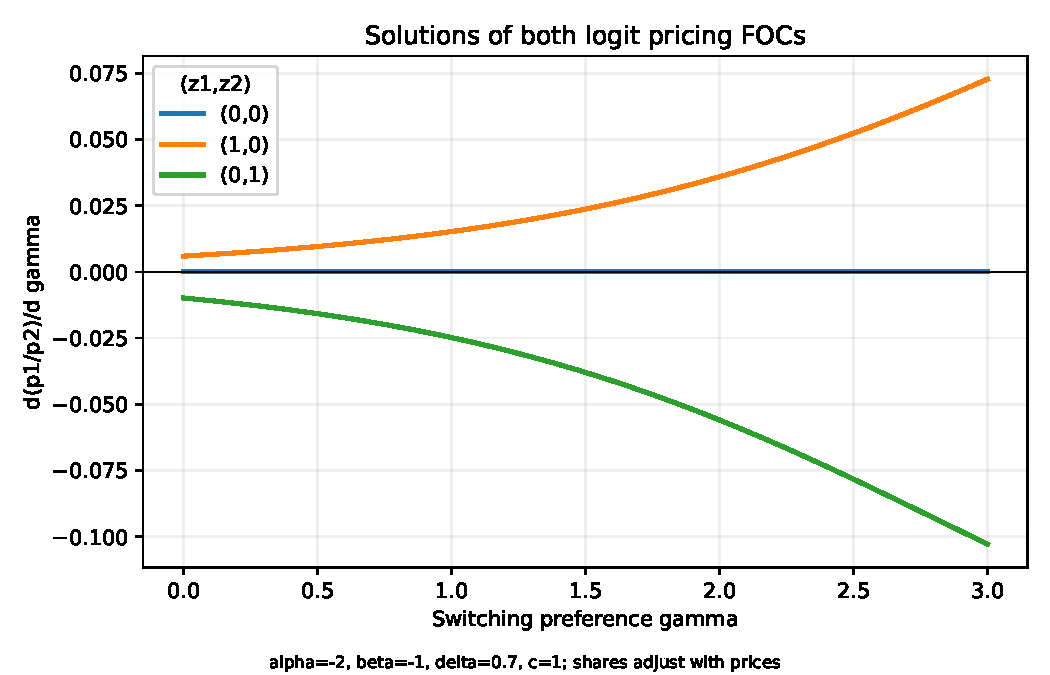
\includegraphics[width=\linewidth]{figures/price_ratio_derivative_cases.pdf}
\end{figure}
\clearpage
\section*{Optimal period-1 price}
\[
p_1^* = c + \frac{\delta s_{2}}{\alpha \left(1 - s_{2}\right)} - \frac{1}{\alpha \left(1 - s_{1}\right)}
\]
\begin{figure}[htbp]
\centering
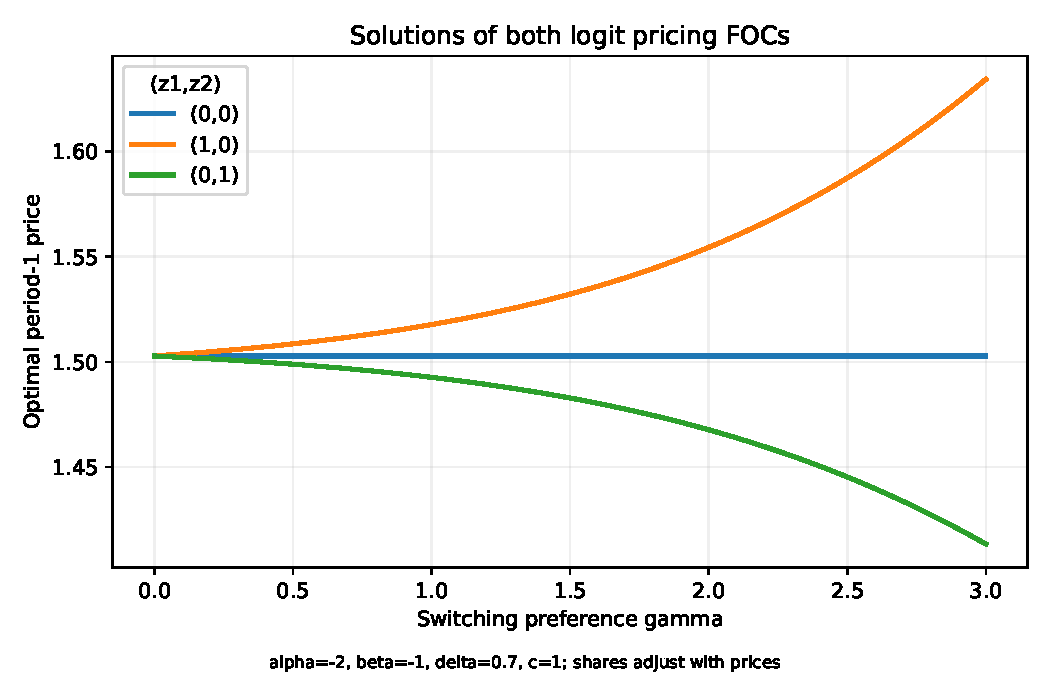
\includegraphics[width=\linewidth]{figures/p1_by_gamma.pdf}
\end{figure}
\clearpage
\section*{Optimal period-2 price}
\[
p_2^* = c - \frac{1}{\alpha \left(1 - s_{2}\right)}
\]
\begin{figure}[htbp]
\centering
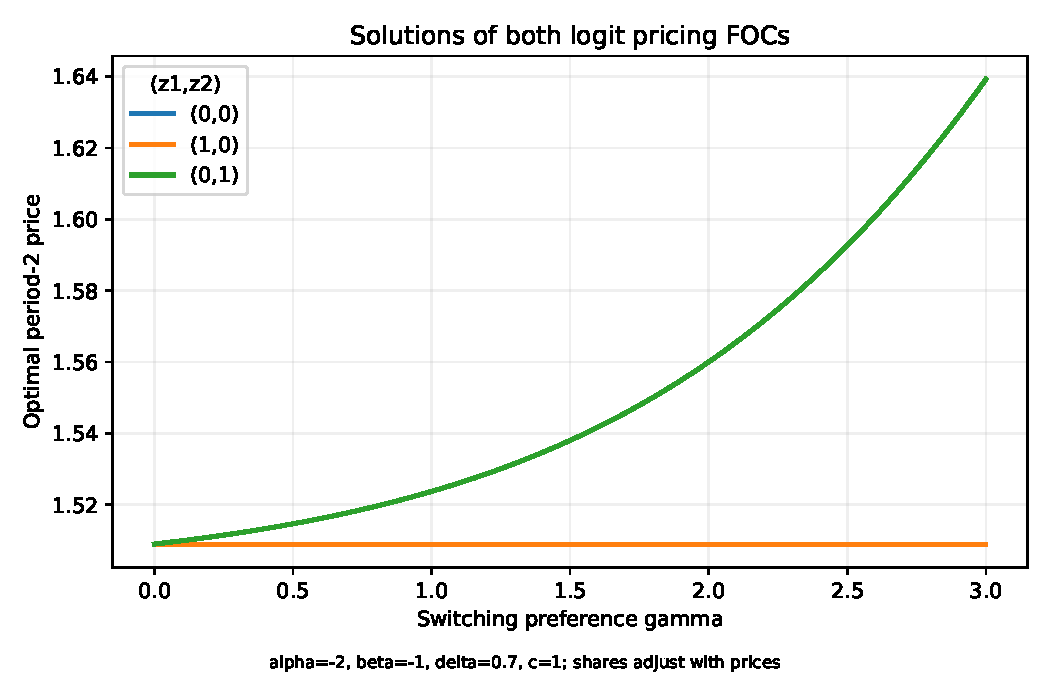
\includegraphics[width=\linewidth]{figures/p2_by_gamma.pdf}
\end{figure}
\clearpage
\section*{$\mathrm{d}^2p_1^*/(\mathrm{d}\gamma\,\mathrm{d}\beta)$}
\[\resizebox{\linewidth}{!}{$\displaystyle \mathrm{d}^2p_1^*/(\mathrm{d}\gamma\,\mathrm{d}\beta) = - \frac{\left(1 - s_{1}\right) \left(\delta^{2} s_{1} s_{2}^{2} z_{2} \left(1 - s_{1}\right) - \delta s_{1}^{2} s_{2} z_{1} + \delta s_{1} s_{2} z_{1} + \delta s_{1} s_{2} z_{2} \left(1 - s_{1}\right) + \delta s_{2}^{2} z_{2} \left(1 - s_{2}\right) - \delta s_{2} z_{2} \left(1 - s_{2}\right) - s_{1}^{2} z_{1} + s_{1} z_{1}\right)}{\alpha}$}\]
\begin{figure}[htbp]
\centering
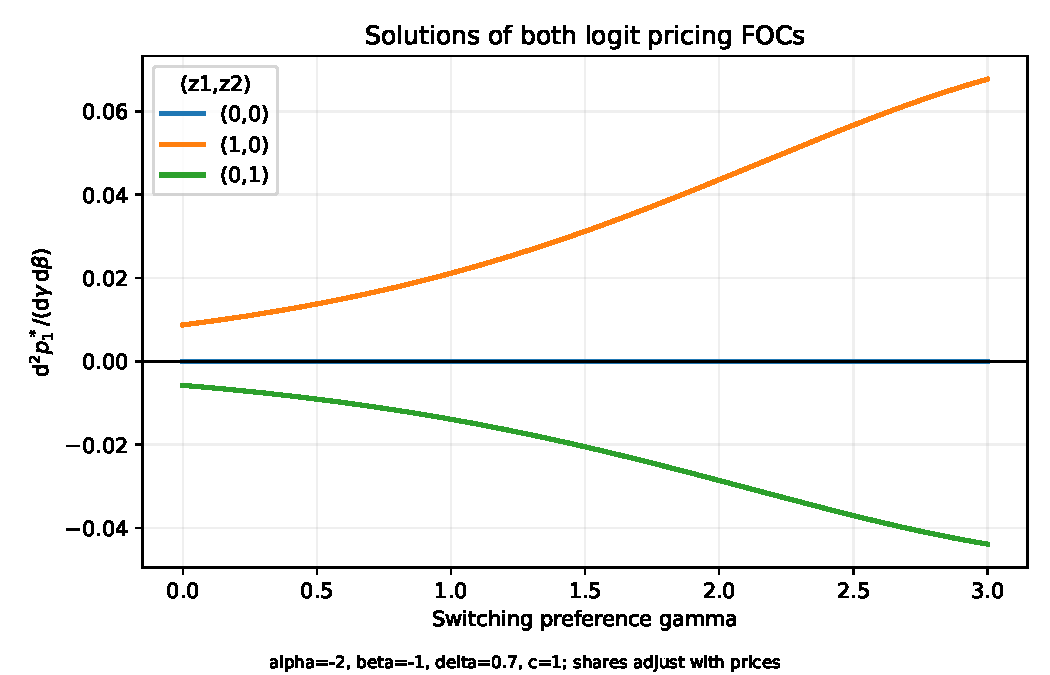
\includegraphics[width=\linewidth]{figures/beta_p1_derivative_by_gamma.pdf}
\end{figure}
\clearpage
\section*{$\mathrm{d}^2p_2^*/(\mathrm{d}\gamma\,\mathrm{d}\beta)$}
\[
\mathrm{d}^2p_2^*/(\mathrm{d}\gamma\,\mathrm{d}\beta) = - \frac{s_{2} z_{2} \left(1 - s_{2}\right)^{2}}{\alpha}
\]
\begin{figure}[htbp]
\centering
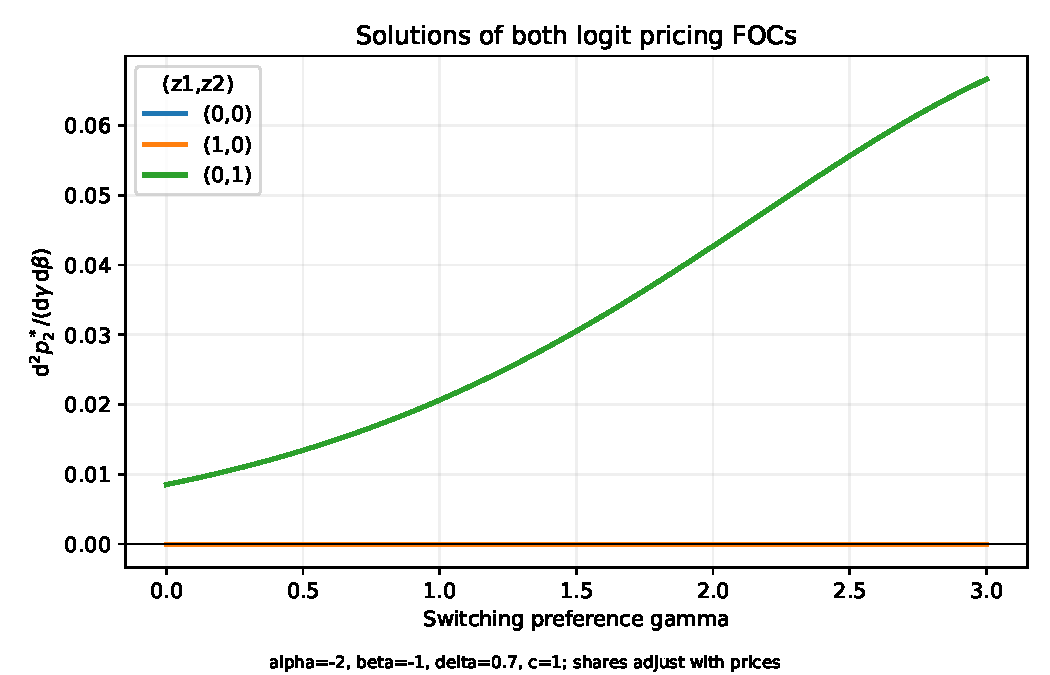
\includegraphics[width=\linewidth]{figures/beta_p2_derivative_by_gamma.pdf}
\end{figure}
\clearpage
\section*{$\mathrm{d}^2p_1^*/\mathrm{d}\gamma^2$}
\[
\mathrm{d}^2p_1^*/\mathrm{d}\gamma^2 = \frac{\delta s_{2} z_{2}^{2} \left(1 - s_{1}\right) \left(1 - s_{2}\right)^{2} - s_{1} \left(1 - s_{1}\right)^{2} \left(\delta s_{2} z_{2} + z_{1}\right)^{2}}{\alpha}
\]
\begin{figure}[htbp]
\centering
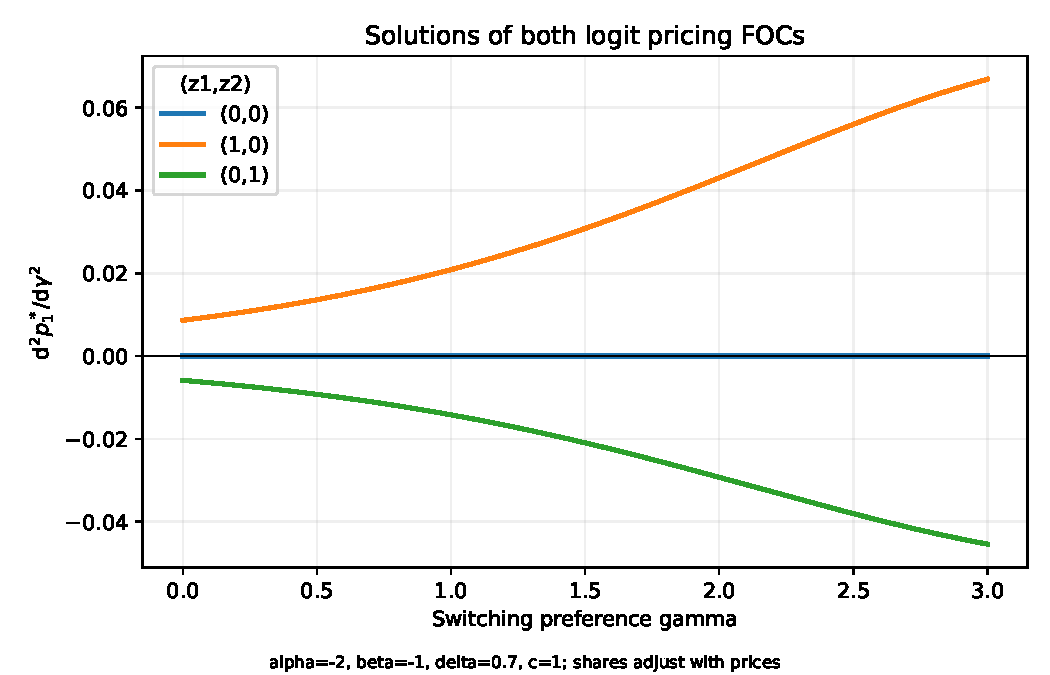
\includegraphics[width=\linewidth]{figures/gamma2_p1_by_gamma.pdf}
\end{figure}
\clearpage
\section*{$\mathrm{d}^2p_2^*/\mathrm{d}\gamma^2$}
\[
\mathrm{d}^2p_2^*/\mathrm{d}\gamma^2 = - \frac{s_{2} z_{2}^{2} \left(1 - s_{2}\right)^{2}}{\alpha}
\]
\begin{figure}[htbp]
\centering
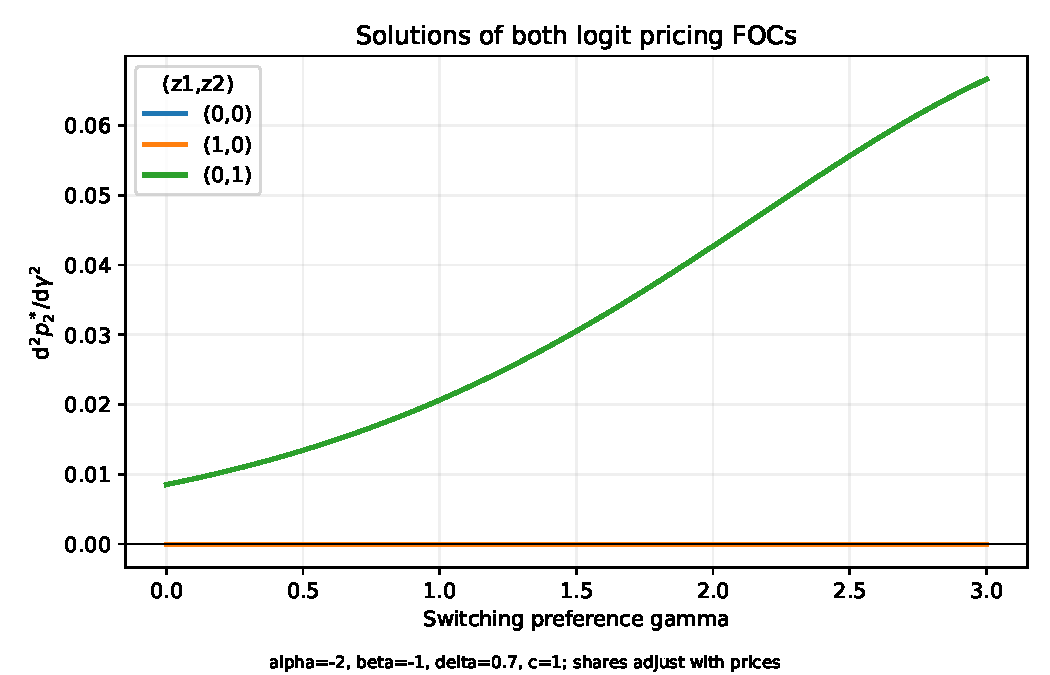
\includegraphics[width=\linewidth]{figures/gamma2_p2_by_gamma.pdf}
\end{figure}
\clearpage
\section*{$\mathrm{d}p_1^*/\mathrm{d}\gamma$}
\[
\mathrm{d}p_1^*/\mathrm{d}\gamma = \frac{\delta s_{2} z_{2} \left(1 - s_{1}\right) - s_{1} z_{1}}{\alpha}
\]
\begin{figure}[htbp]
\centering
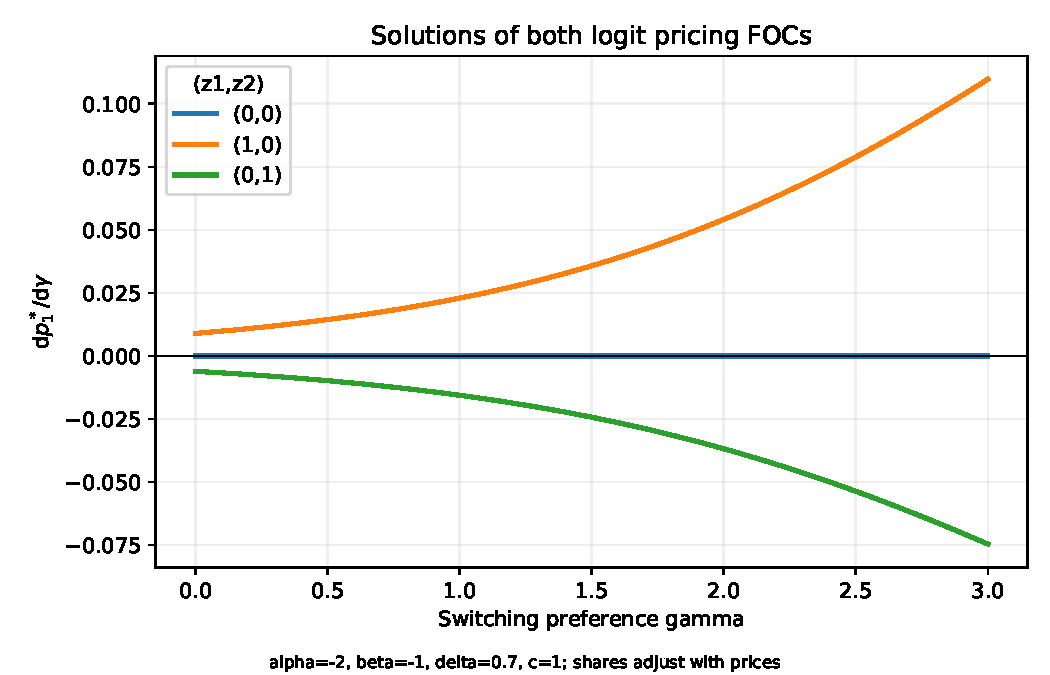
\includegraphics[width=\linewidth]{figures/gamma_p1_by_gamma.pdf}
\end{figure}
\clearpage
\section*{$\mathrm{d}p_2^*/\mathrm{d}\gamma$}
\[
\mathrm{d}p_2^*/\mathrm{d}\gamma = - \frac{s_{2} z_{2}}{\alpha}
\]
\begin{figure}[htbp]
\centering
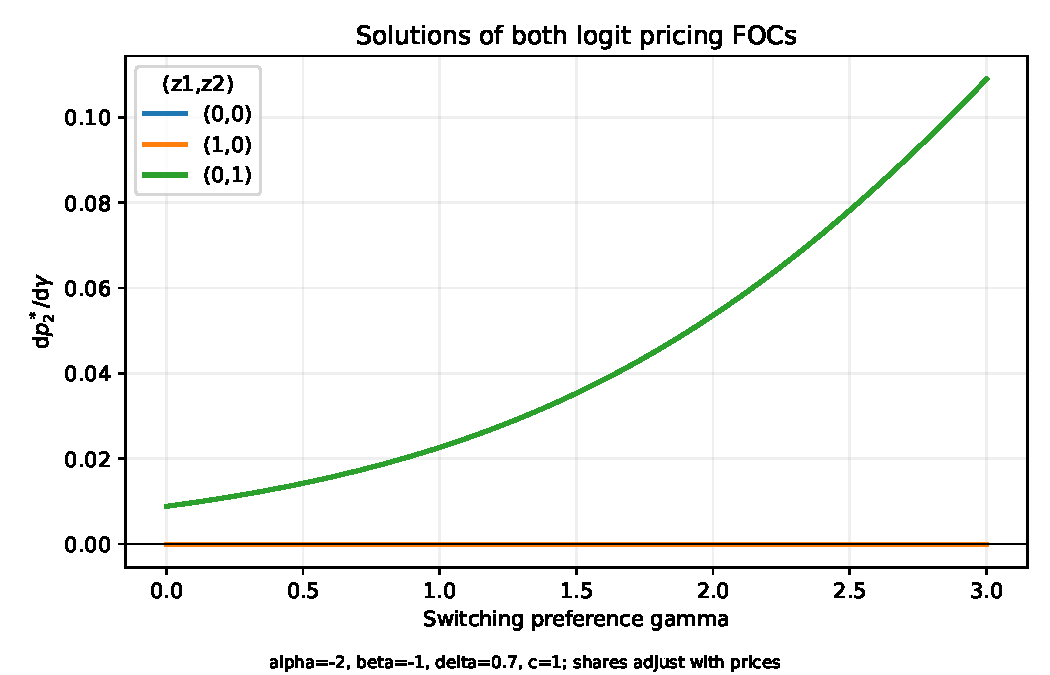
\includegraphics[width=\linewidth]{figures/gamma_p2_by_gamma.pdf}
\end{figure}
\clearpage
\section*{$\mathrm{d}p_1^*/\mathrm{d}\beta$}
\[
\mathrm{d}p_1^*/\mathrm{d}\beta = \frac{\delta s_{2} \left(1 - s_{1}\right) - s_{1}}{\alpha}
\]
\begin{figure}[htbp]
\centering
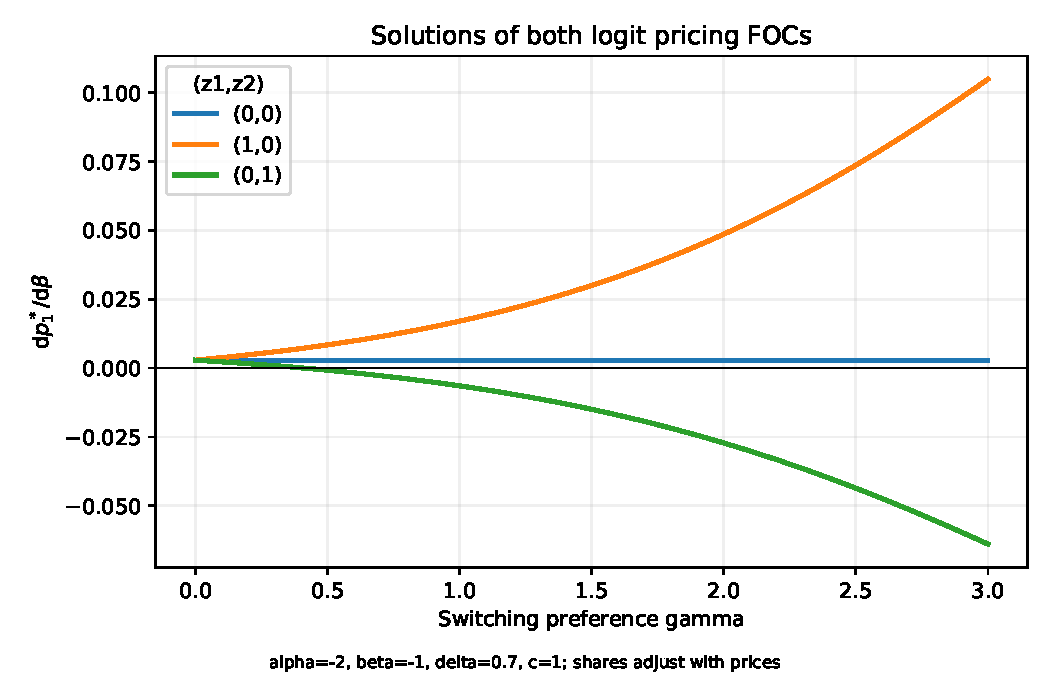
\includegraphics[width=\linewidth]{figures/beta_p1_by_gamma.pdf}
\end{figure}
\clearpage
\section*{$\mathrm{d}p_2^*/\mathrm{d}\beta$}
\[
\mathrm{d}p_2^*/\mathrm{d}\beta = - \frac{s_{2}}{\alpha}
\]
\begin{figure}[htbp]
\centering
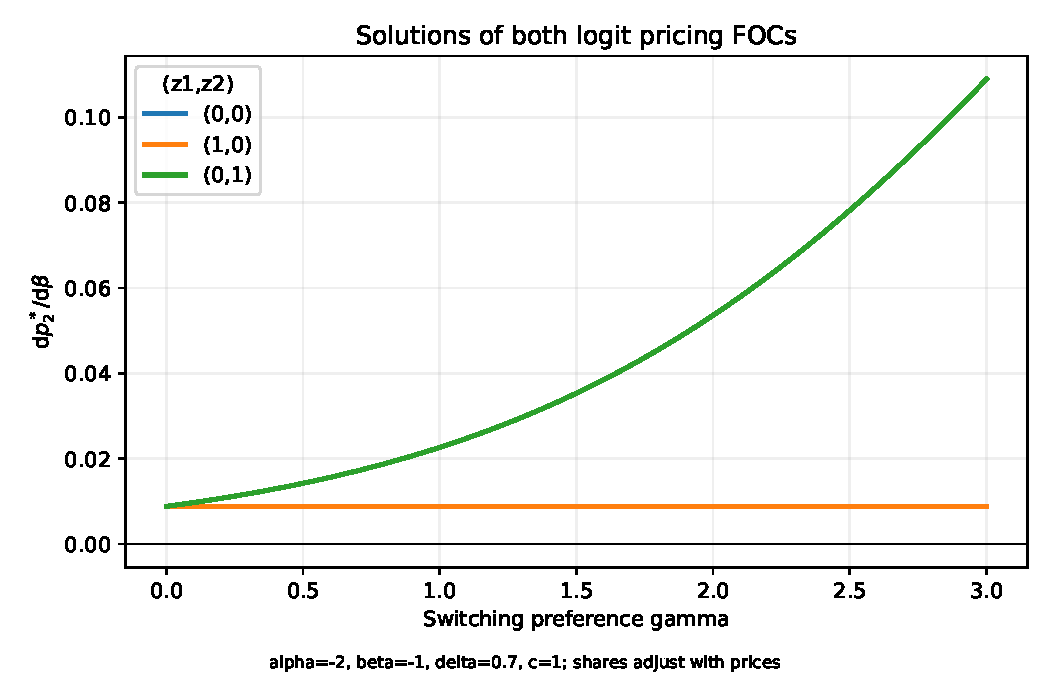
\includegraphics[width=\linewidth]{figures/beta_p2_by_gamma.pdf}
\end{figure}
\clearpage
\section*{$\mathrm{d}p_1^*/\mathrm{d}\alpha$}
\[
\mathrm{d}p_1^*/\mathrm{d}\alpha = \frac{\delta p_{2} s_{2} \left(1 - s_{1}\right)}{\alpha} - \frac{p_{1} s_{1}}{\alpha} + \frac{1}{\alpha^{2}}
\]
\begin{figure}[htbp]
\centering
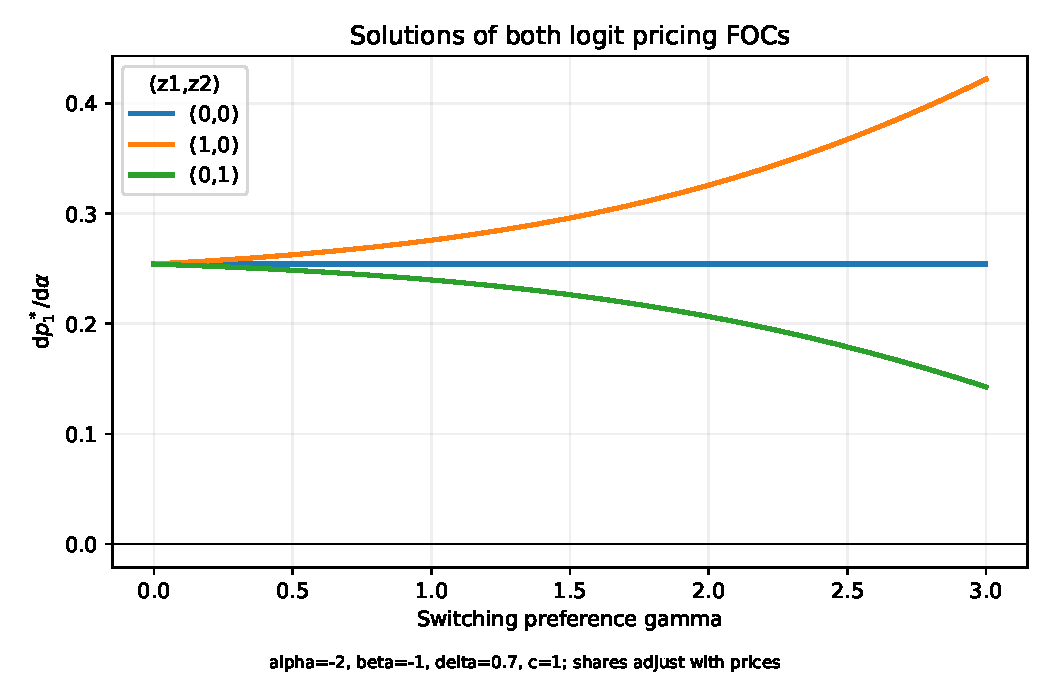
\includegraphics[width=\linewidth]{figures/alpha_p1_by_gamma.pdf}
\end{figure}
\clearpage
\section*{$\mathrm{d}p_2^*/\mathrm{d}\alpha$}
\[
\mathrm{d}p_2^*/\mathrm{d}\alpha = \frac{- \alpha p_{2} s_{2} + 1}{\alpha^{2}}
\]
\begin{figure}[htbp]
\centering
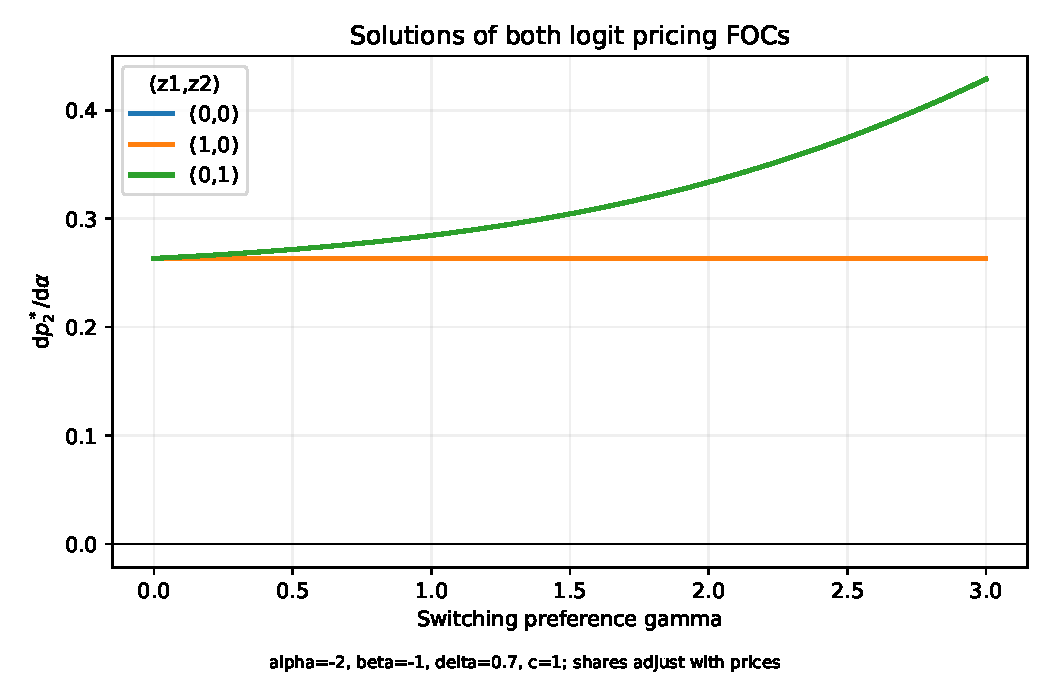
\includegraphics[width=\linewidth]{figures/alpha_p2_by_gamma.pdf}
\end{figure}
\clearpage
\section*{$\mathrm{d}p_1^*/\mathrm{d}\delta$}
\[
\mathrm{d}p_1^*/\mathrm{d}\delta = \frac{s_{2} \left(1 - s_{1}\right)}{\alpha \left(1 - s_{2}\right)}
\]
\begin{figure}[htbp]
\centering
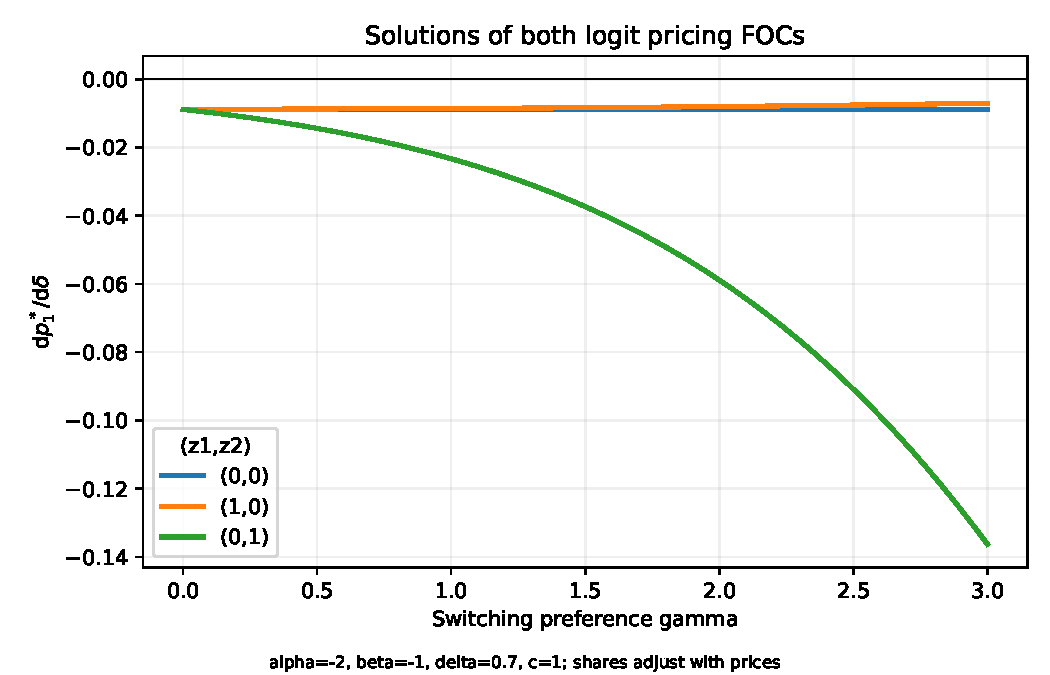
\includegraphics[width=\linewidth]{figures/delta_p1_by_gamma.pdf}
\end{figure}
\clearpage
\section*{$\mathrm{d}p_2^*/\mathrm{d}\delta$}
\[
\mathrm{d}p_2^*/\mathrm{d}\delta = 0
\]
\begin{figure}[htbp]
\centering
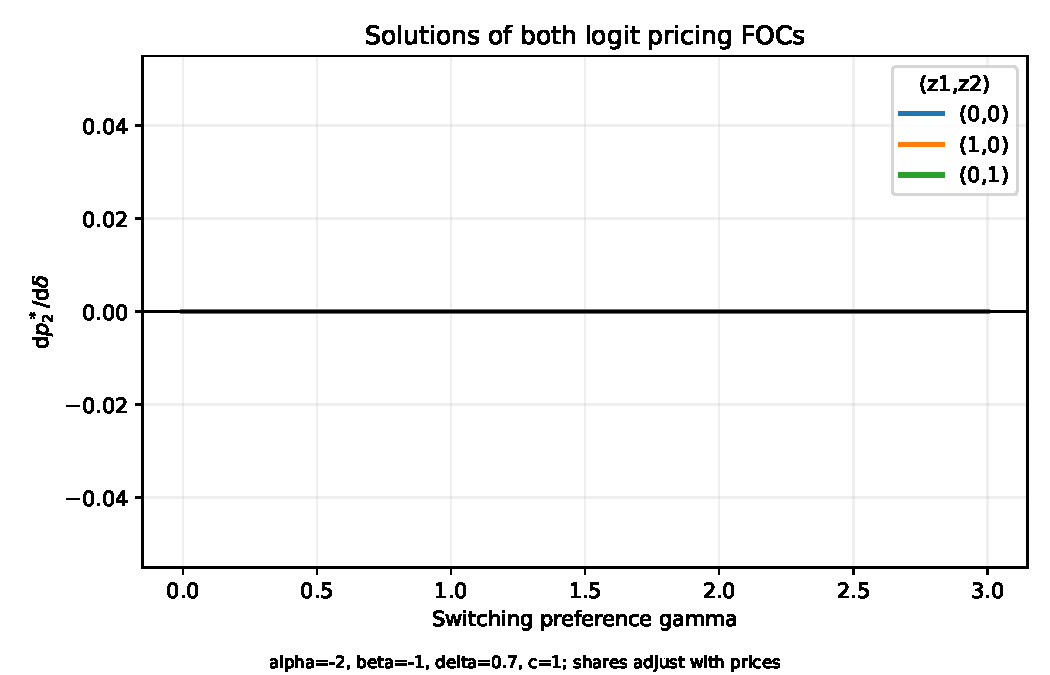
\includegraphics[width=\linewidth]{figures/delta_p2_by_gamma.pdf}
\end{figure}
\clearpage
\section*{$\mathrm{d}\Pi^*/\mathrm{d}\gamma$}
\[
\mathrm{d}\Pi^*/\mathrm{d}\gamma = - \frac{s_{1} \left(\delta s_{2} z_{2} + z_{1}\right)}{\alpha}
\]
\begin{figure}[htbp]
\centering
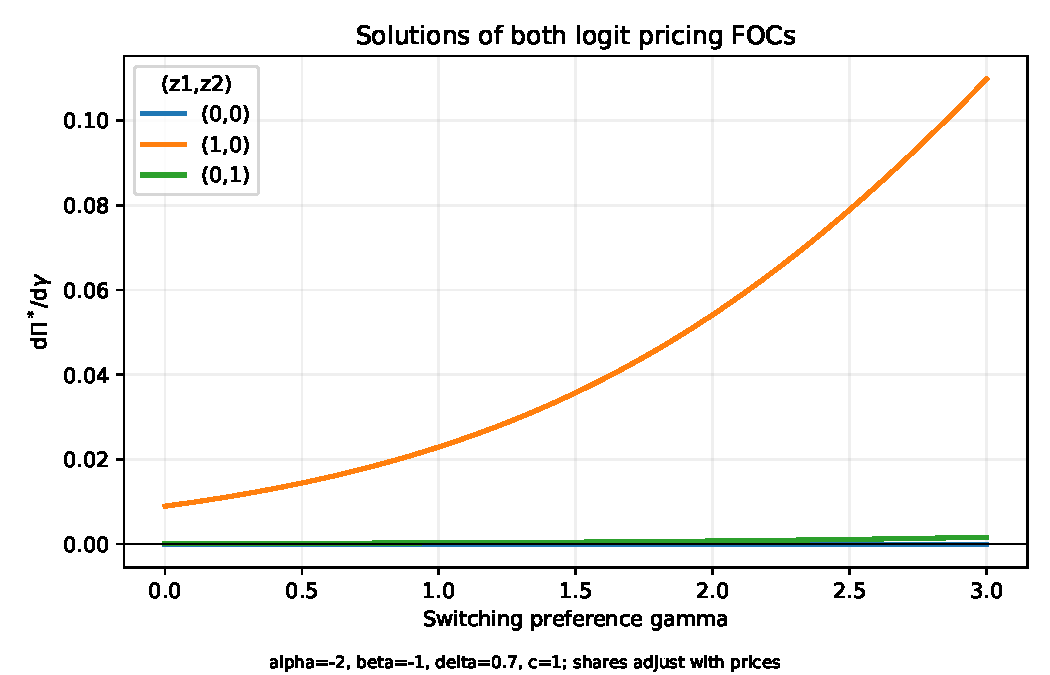
\includegraphics[width=\linewidth]{figures/gamma_profit_by_gamma.pdf}
\end{figure}
\clearpage
\section*{$\mathrm{d}(p_1^*/p_2^*)/\mathrm{d}\beta$}
\[
\mathrm{d}(p_1^*/p_2^*)/\mathrm{d}\beta = \frac{\frac{p_{1} s_{2}}{\alpha} + \frac{p_{2} \left(\delta s_{2} \left(1 - s_{1}\right) - s_{1}\right)}{\alpha}}{p_{2}^{2}}
\]
\begin{figure}[htbp]
\centering
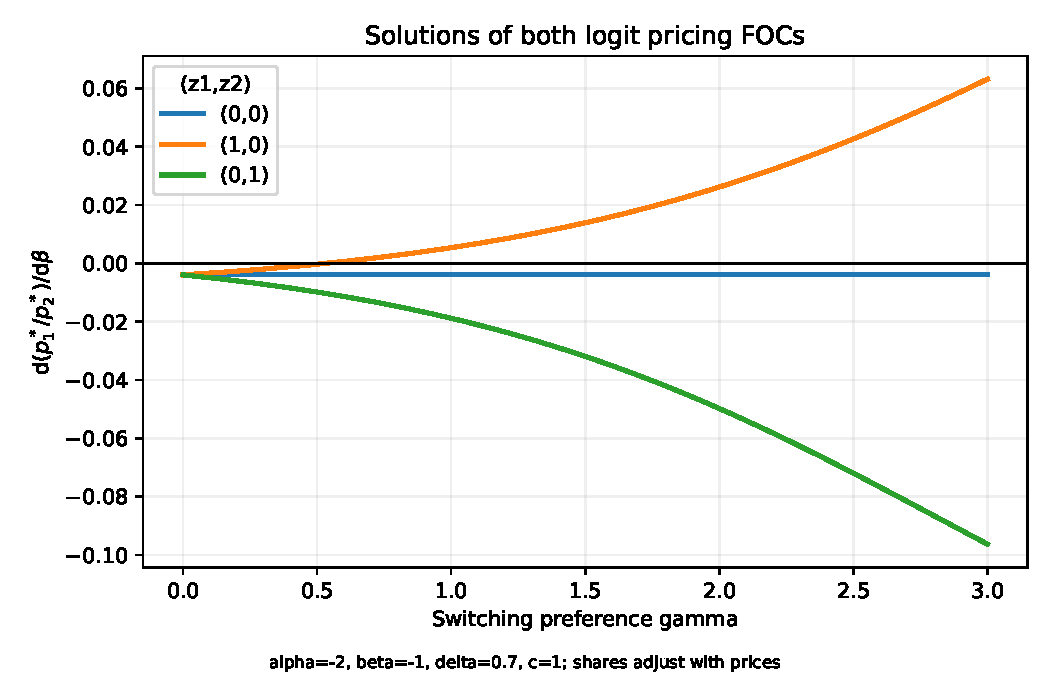
\includegraphics[width=\linewidth]{figures/beta_price_ratio_by_gamma.pdf}
\end{figure}
\clearpage
\section*{Period-1 pricing condition}
\[
F_1 = \alpha s_{1} \left(1 - s_{1}\right) \left(- c + \delta s_{2} \left(- c + p_{2}\right) + p_{1}\right) + s_{1}
\]
\begin{figure}[htbp]
\centering
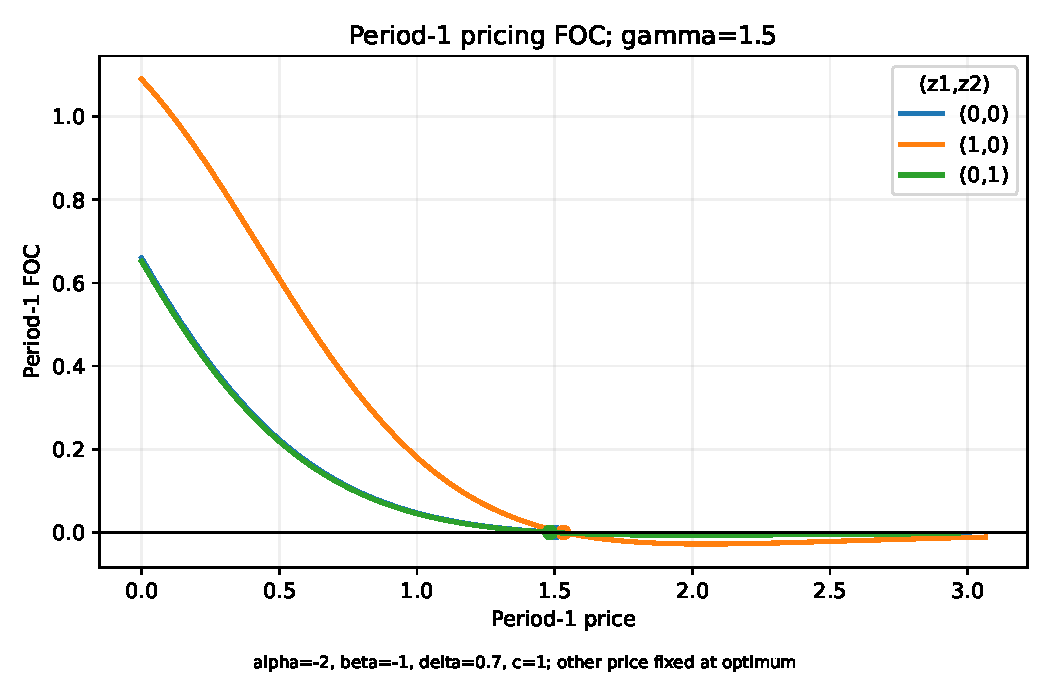
\includegraphics[width=\linewidth]{figures/period1_foc.pdf}
\end{figure}
\clearpage
\section*{Period-2 pricing condition}
\[
F_2 = - \alpha c s_{2} \left(1 - s_{2}\right) + \alpha p_{2} s_{2} \left(1 - s_{2}\right) + s_{2}
\]
\begin{figure}[htbp]
\centering
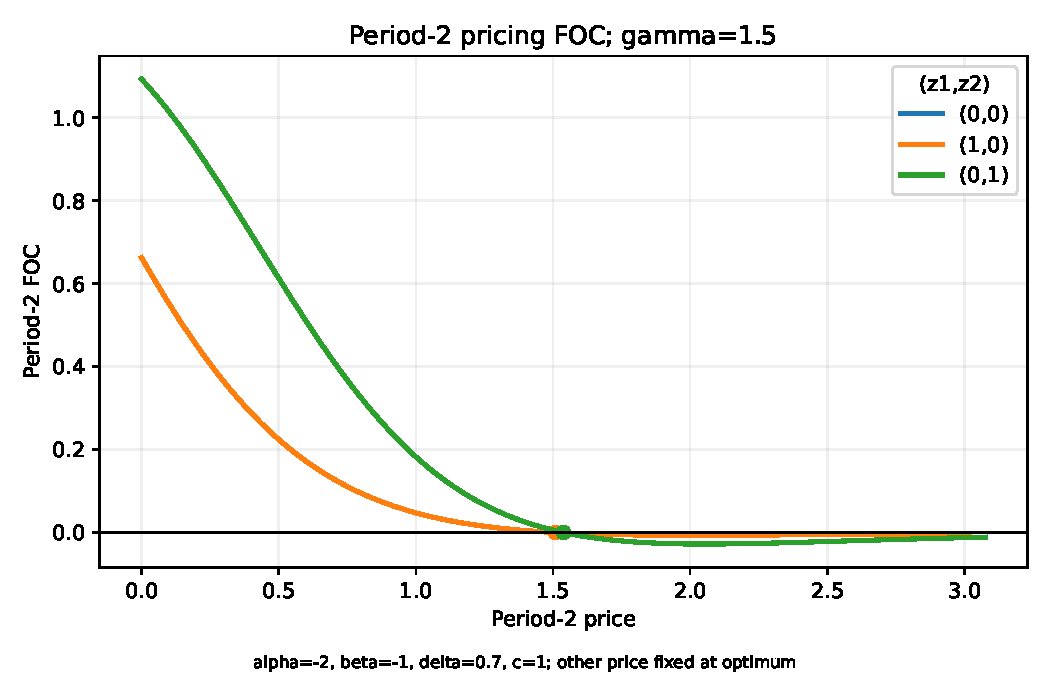
\includegraphics[width=\linewidth]{figures/period2_foc.pdf}
\end{figure}
\end{document}
